\documentclass{ujarticle}
\usepackage{robomech2022}
\usepackage[dvipdfmx]{graphicx}

\begin{document}
\makeatletter
\title{ROSロボットと連動するVOD型e-Learningシステムの実現}
{}
{Implementing an e-Learning VOD system linked with actual ROS robot}
{}

\author{
\begin{tabular}{ll}
 \hspace{1zw}◯学\hspace{1zw}瀧本 恒平 (はこだて未来大)& \hspace{1zw} 松原 克弥(はこだて未来大)\\
 \hspace{1zw}正\hspace{1zw}鈴木 昭二(はこだて未来大)\\
 % ※協賛・後援団体の会員資格で発表される場合は「正・学」は不要です。
 &\\
 \multicolumn{2}{l}{\small Kouhei TAKIMOTO, Future University Hakodate, g2121032@fun.ac.jp}\\
 \multicolumn{2}{l}{\small Katsuya MATSUBARA, Future University Hakodate}\\
 \multicolumn{2}{l}{\small Sho'ji SUZUKI, Future University Hakodate}\\
\end{tabular}
}
\makeatother

\abstract{ \small
ROS, an open source robot control software platform, is widely used for robot development. Accordingly, robot development engineers are required to have skills in robot control programming using ROS, but in most of the existing ROS-learning contents, it is not possible to confirm that the program and the robot are running in synchronization in the real world at hand. Therefore, we may lose the significance of checking at hand, such as understanding the difference between the virtual world and the physical world. In this study, we propose an e-Learning system for ROS programming that links a lecture-style video with an actual robot at hand. By measuring the latency from the time the video is played to the time the actual robot at hand starts to move, we demonstrated the practicality of the system and summarized the problems and future prospects.
}

\date{} % 日付を出力しない
\keywords{Robot Operating System(ROS), e-Learning, actual robot}

\maketitle
\thispagestyle{empty}
\pagestyle{empty}

\small
\section{はじめに}%===========================
OSSロボット制御ミドルウェアであるRobot Operating System(ROS)は,開発をサポートする豊富なツール,再利用性の高いパッケージ群やそれらを柔軟に組み合わせるためのノードグラフ・モデルの採用により,多くのロボットシステムで採用が進んでいる.
ROSの普及にともなって,ROSを用いたロボット制御プログラミングのスキルを持つエンジニアの需要が高まっている.
実際,これに対応するように,ROSを用いたロボット制御プログラミングの学習教材や学習環境が充実してきている.
コンピュータ上で動作させる通常のプログラミングと比較して,ロボット制御プログラミングでは,プログラミング言語やAPI等の理解だけでなく,ロボットの物理的な装置の挙動について意識する必要がある.
ロボットの物理的な装置の挙動で意識するべき点とは,ロボットが移動する際の加速度や,ロボットが移動した際にバランスを保ったまま移動できているかどうか等を指す.
しかし,ロボット制御プログラミングに関する既存の学習教材の多くは,プログラムコードやその解説が記述されたテキスト形式のコンテンツが主体となっているため,教材が対象としているロボットの物理的な装置の挙動を伝えることや,その挙動を意識しながら学習することが難しいという課題がある.
\par また,コロナ禍における対面教育の制限にともなって,プログラミング学習に対するe-Learningの需要が拡大している.
e-Learningによる学習は,教材の質が均一であり,講師毎の違いに左右されず,時間と場所を選ばずに繰り返し学習できることがメリットである.
一方,e-Learningによる学習では,学習を継続するためのモチベーションの維持が難しいことや,本研究が対象とするロボット制御のような,実習・実技をともなう学習を十分にサポートすることが難しいという課題が存在する.
ロボット制御プログラミング向けの既存e-Learning教材では,ロボットを動かしている様子を撮影した動画やCGで再現した仮想ロボットを使ってロボットの挙動を解説しているものが多く,前述の学習モチベーションの維持や,実世界におけるロボットの挙動を意識するという点において,動画やCGだけではロボットの挙動を解説する方法として十分とは言えない.
\par 本研究では,ロボット制御プログラミングを対象としたe-Learningにおいて,学習モチベーションの向上と実勢会でのロボット挙動を意識した学習の実現を目的として,講義形式の動画の解説に合わせて手元のロボットが連動し,ロボット内で動作しているプログラムの状態理解を支援するシステムを提案する.
提案システムの概要を,図\ref{fig:Proposal_system_ab}に示す.
学習者は,ロボットの挙動とプログラムコードを解説した動画をWebブラウザ内で視聴することで学習を進めると同時に,視聴している動画が指定されたタイミングまで進むと,Webブラウザ上で対応するロボット制御プログラムが実行され,手元にある実機ロボットが動画と連動して動作する.
これにより,プログラムとロボットが実世界で同期して動いていることを手元で確認しつつ,e-Learningの持つメリットである,時間と場所を問わずに繰り返し学習できることと教材の質が均一であることを活かした学習ができるようになる.

\begin{figure}[t]
  \centering
  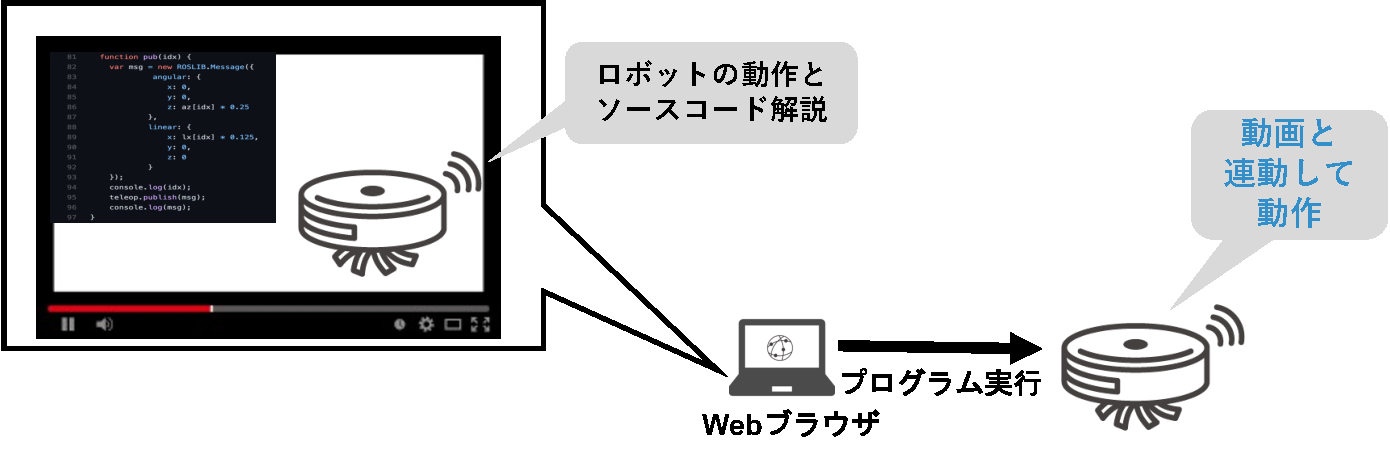
\includegraphics[keepaspectratio, scale=0.3]{./src/Proposal_system_ab.pdf}
  \caption{Overview of the proposed system}
  \label{fig:Proposal_system_ab}
\end{figure}

\section{既存のe-Learningシステムの課題}
本章では,既存のロボット制御プログラミングを学習可能なe-Learningシステムを3つ紹介した後で,それらの抱える課題について述べる.
\par 第一にUdemy\cite{Udemy}というサービスがある.Udemyは,オンラインの学習プラットフォームであり,専門的な知識を解説したスライドや,ソースコードを記述しながら口頭で解説している様子に加え,その実行結果を記録した動画を用いて学習できる.
\par 第二にThe Construct\cite{Construct}というサービスがある.The Constructは,ソースコードや専門的な知識を解説したテキストを閲覧しつつ,ブラウザ上に用意された仮想開発環境でコマンドやソースコードの記述を行い,シミュレータ上でロボットを動作させることができるオンライン学習サービスである.また,実機ロボットの操作権限を事前に予約しておくことで,The Constructが所有している実機ロボットをカメラ越しに動作させることもできる.
\par 第三にGustavoらの研究で提案されているロボット制御プログラミングの学習支援システム\cite{Gustavo}がある.この研究では,Webブラウザ上でROSのソースコードを記述し,プログラムを実行することで,Webブラウザ上にシミュレータの動作や出力結果を表示するシステムを提案している.提案の実現により,学習者は開発環境の構築や,コンパイル等の手間を掛けずにロボット制御プログラミングを学習できる.
\par これらの既存のロボット制御プログラミングを学習可能なe-Learningシステムでは,動画やシミュレータを用いてロボットの物理的な装置の挙動を確認するようにしているが,動画やシミュレータによるロボットの動作確認は,プログラムとロボットが実世界で同期して動いていることを手元で確認できないという課題がある.ロボットを手元で確認する意義には,
\begin{itemize}
  \item 仮想的な世界と物理的な世界の違いを理解すること
  \item 現実のものが動くことによる面白さ
  \item ハードウェアの仕組みに関する関心が深まること
  \item 学習してきた物理・数学が実世界とどう関わっているか知ること
  \item ロボット本体と周辺環境に触れて試行錯誤すること
\end{itemize}
等がある.これらのロボットを手元で確認する意義は,実機があるからこそ学ぶことができるものであり,仮想的な世界のみでは得ることができない.


\section{提案}
動画やスライドといった順序型コンテンツと実機デバイスの連動によりプログラミング学習の支援を行っている研究として,川谷らの研究\cite{Kawatani}がある.この研究では,Web上に存在するIoTプログラミング学習が可能な順序型コンテンツに対して,コンテンツの順序に応じたプログラムを埋め込むことで,特定のタイミングでソースコードの表示やIoTデバイスの制御が可能なシステムを提案している.提案の実現により,順序型コンテンツ内のIoTデバイスと手元のIoTデバイスが連動することで,学習者のIoTデバイスに対する理解度と学習意欲の向上を図っている.
\par 本論文では,川谷らの研究から着想を得て,動画と実機ロボットが手元で連動することで,ロボット制御プログラミング学習の支援を行うシステムを提案する.提案システムでは,動画の再生位置に基づいて,手元の実機ロボットの制御を行い,制御に用いられた制御コマンドをブラウザ上で確認できるようになっている.ユーザは,動画内のロボットやソースコードの解説と連動した実機ロボットの動作を見ることができるため,動画やシミュレータのみで学習するよりもロボットの物理的な装置の挙動について理解しやすくなる.また,手元の実機ロボットが動作した際の制御コマンドを確認することが出来るため,ユーザ自身で同様のプログラムを再現しやすくなる.想定されるシステムの利用ケースとして,ユーザがPCでロボット制御プログラミング学習動画を視聴している際,動画内のロボットが前進すると,ユーザの手元にある実機ロボットも連動して前進する.その際,動画を視聴しているブラウザ上にリアルタイムで制御コマンドが表示される.
\par 提案システムに必要な要件として,以下の2つがある.

\begin{enumerate}
  \item 実機ロボットがユーザの手元で動作すること
  \item ロボットの動作に用いた制御コマンドを表示すること
\end{enumerate}

要件1は,動画内でロボットの動作を見るだけでなく,実際に手元の実機ロボットが動作している様子を確認することで,ロボットの物理的な装置の挙動に関する理解度の向上や,学習に対するモチベーションの向上に繋がるため設定した.要件2は,ユーザが実際にロボット開発を進める時に,動画の再生位置のどの部分でロボットにどのような制御コマンドが送信されていたのかを知ることで,ロボットの動作に要するセンサの値について理解しやすくなるため設定した.本論文では,これらの要件を満たすシステムを構築する.


\section{実装}
本論文では,動画と手元の実機ロボットを連動させる機能を実装する.実装するシステム構成図を図\ref{fig:Implemented_system}に示す.学習コンテンツとして用いる動画に埋め込むプログラムと動画コンテンツを外部でホスティングされているサーバから受け取り,受け取った学習コンテンツを実行するWebブラウザとロボットの通信を仲介するローカルサーバを構築することで,動画と手元の実機ロボットの連動を実現する.

\begin{figure}[t]
  \centering
  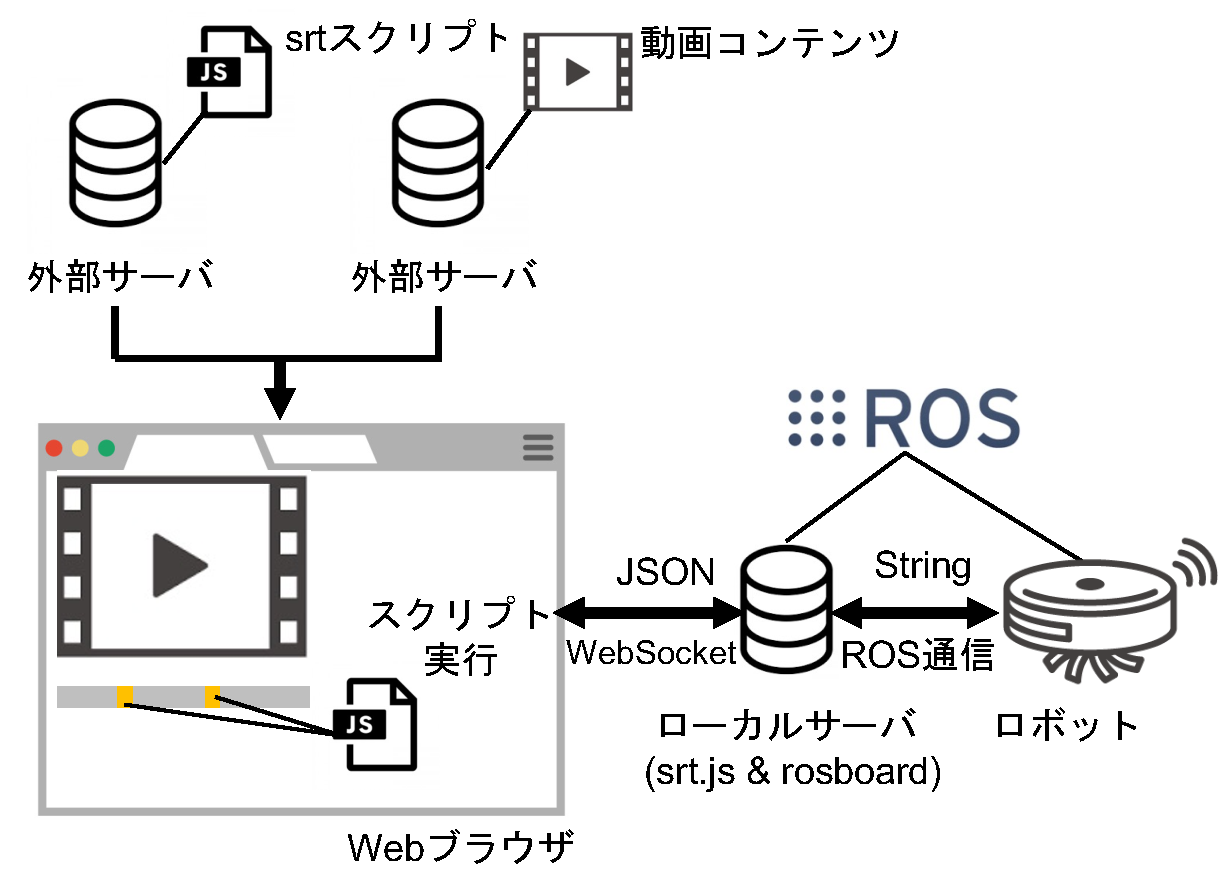
\includegraphics[keepaspectratio, scale=0.4]{./src/Implemented_system.pdf}
  \caption{System configuration}
  \label{fig:Implemented_system}
\end{figure}

\par 動画と手元の実機ロボットの連動の実現を行うには,動画にプログラムを埋め込み,動画の再生位置に合わせてプログラムを実行する機能の実装とWebブラウザからロボットに制御コマンドを送信する機能の実装に加え,提案システムに対応したROS学習動画に埋め込むプログラムの記述に関する制約を設定する必要がある.
\par 動画にプログラムを埋め込み,動画の再生位置に合わせてプログラムを実行する機能の実装には,srt.js\cite{srt.js}を用いる.srt.jsは,YouTube等の映像コンテンツの字幕形式として公式にサポートされているsrtファイルの形でJavaScriptを埋め込むことができ,動画上の再生位置に応じてプログラムを実行できるフレームワークである.図\ref{fig:srt_example}にsrtスクリプトの記述例を示す.srtスクリプトには,動画上の再生位置を記述し,そのタイミングで実行したいJavaScriptプログラムを記述する.これにより,動画の再生位置に合わせてプログラムを実行する機能が実現される.
\par ただし,動画を一時停止してもプログラムの実行が停止されないことや,動画をスキップした際にsrtスクリプトで指定した動画の再生位置を超えてしまうとそのプログラムを実行できないことがある.そのため,手元の実機ロボットが動画内で想定されている動作以上の範囲で動作してしまうことや,ユーザが動画に対して行うスキップ等の操作を制限してしまうことになる.この課題を解決するために,ユーザが動画に対して行う操作で考えられるケースについて検討し,それぞれに応じた処理を追加した.ユーザが動画に対して行う操作として,以下の3つが考えられる.

\begin{figure}[t]
  \centering
  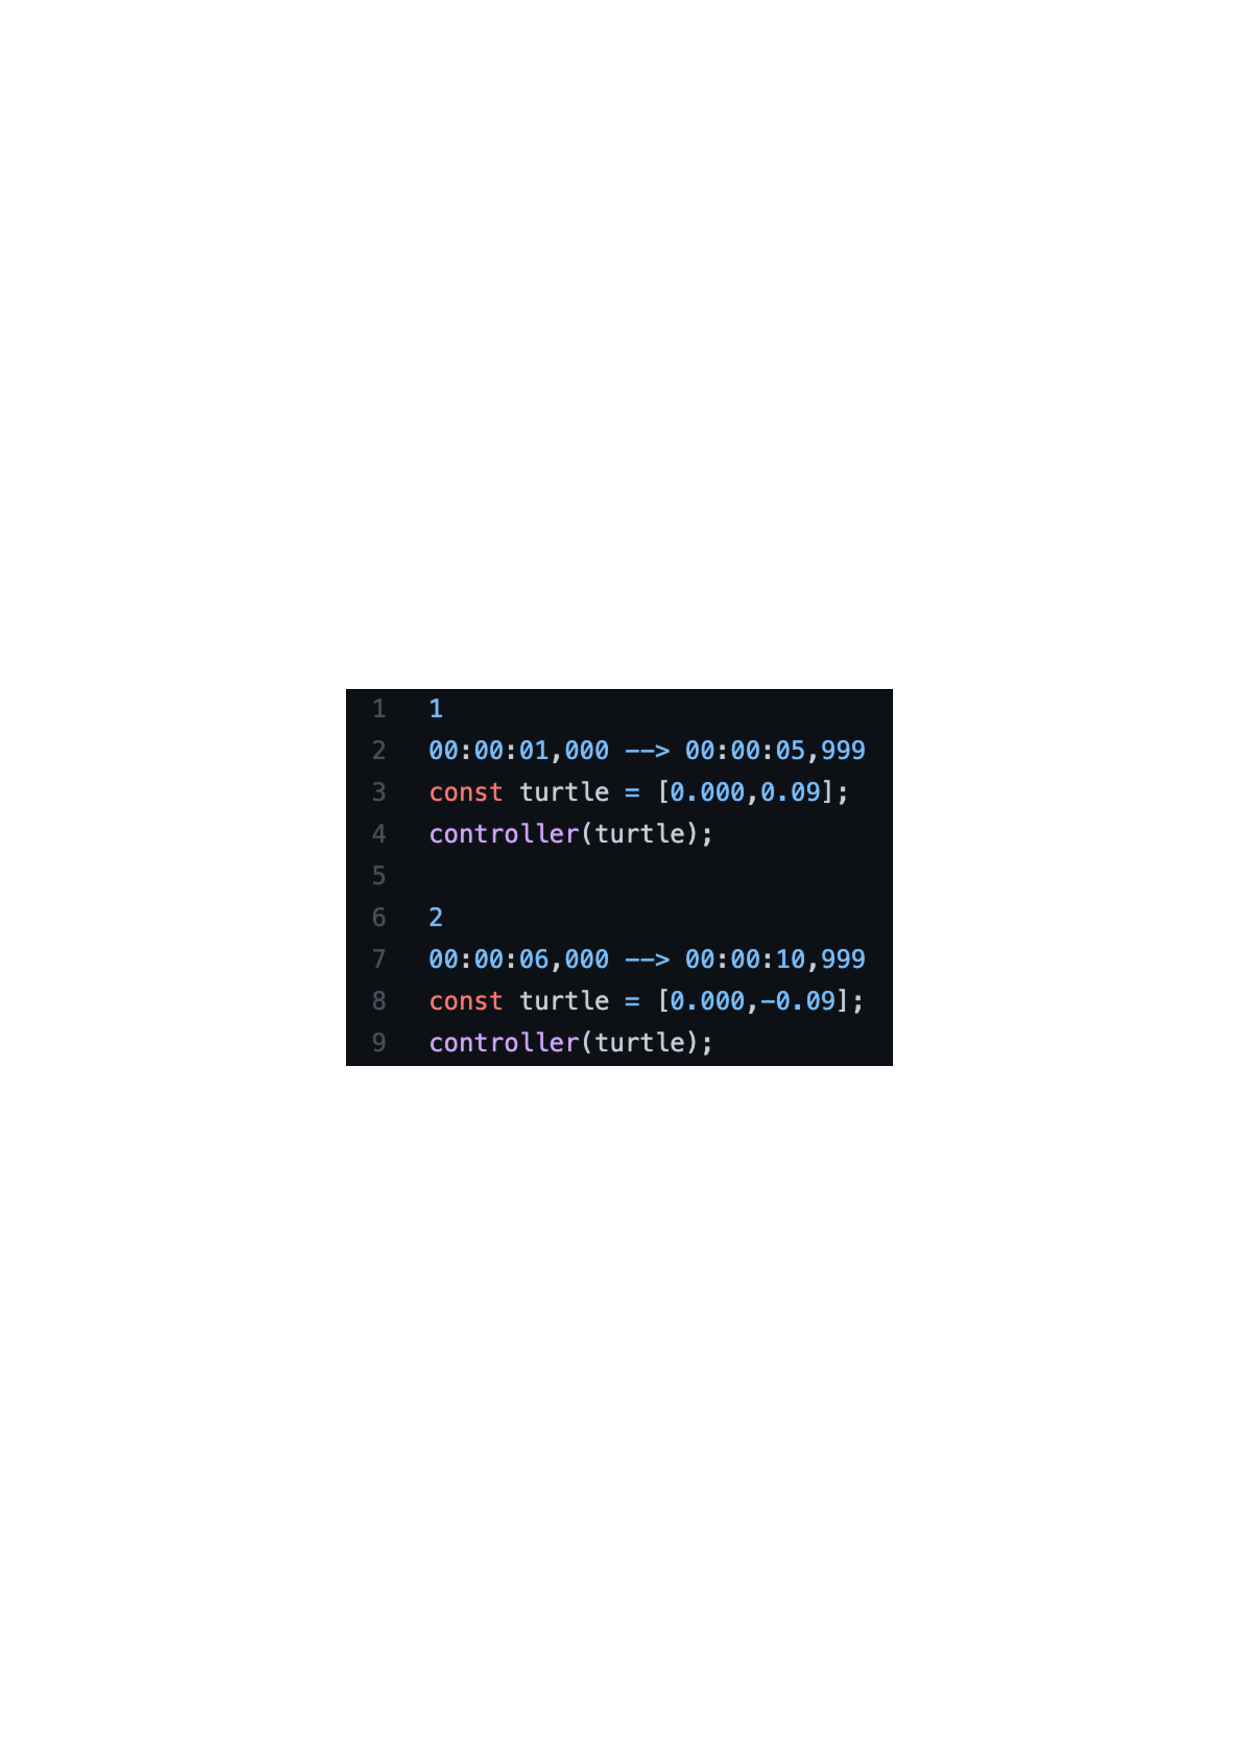
\includegraphics[keepaspectratio, scale=0.7]{./src/srt_example.pdf}
  \caption{Example of srt script description}
  \label{fig:srt_example}
\end{figure}

\begin{enumerate}
  \item 動画が最初から最後まで通して再生された
  \item 動画が一時停止された
  \item 動画が前後どちらかにスキップされた
\end{enumerate}

\par 1つ目のケースに関して,動画の再生状態が終了に変化した時,実機ロボットの動作を停止させる制御コマンドを送信する処理を追加することで,srtスクリプトにロボットを停止させるスクリプトが含まれていなかった場合であっても,ロボットを停止させることができるようにした.
\par 2つ目のケースに関して,動画の再生状態が一時停止に変化した時,実機ロボットの動作を停止させる制御コマンドを送信する処理を追加することで,動画を一時停止してもプログラムの実行が停止されず,ロボットが動き続けてしまうという課題を解決した.また,動画の再生状態が一時停止から再生中に戻った時,一時停止前に実行していたスクリプトを再度読み込んで実行する処理を追加することで,一時停止状態から復帰した際に再びロボットを動作させることができるようにした.
\par 3つ目のケースに関して,動画の再生中に再生位置がスキップされる際,必ずバッファリングが発生することから,バッファリングが発生した時に実機ロボットの動作を停止させる制御コマンドを送信する処理を追加することで,動画のスキップ中にロボットが動作することを防ぎつつ,スキップ先の再生位置で指定されているスクリプトの実行ができるようにした.
\par これらの処理を実装することで,手元の実機ロボットの想定外の動作を防ぎつつ,ユーザは自分のペースで動画を用いた学習ができるようになる.


\par Webブラウザからロボットに制御コマンドを送信する機能の実装には,rosboard\cite{rosboard}を用いる.rosboardは,ROSロボットが送受信するデータをブラウザ上で可視化でき,ブラウザとROSロボット間での通信もサポートできるフレームワークであり,Webサーバを実行するROSノードである.他のブラウザとROSロボット間の通信をサポートするフレームワークと比較して,通信をサポート可能なROSのバージョンが幅広いことや,ROSノード間で通信されるデータの可視化までサポートしていることから,本研究で扱うWebブラウザとROSロボット間の通信をサポートするフレームワークとして選択した.rosboardは,WebSocket通信により,ブラウザからROSノードに対して同期的にデータを送信する.このとき,ロボットを動作させるためにブラウザから送信されるデータの整形や処理を追加することで,srtスクリプトの作成者や提案システムのユーザがデータ形式の違いを意識することなく,Webブラウザとロボット間で通信が可能となる.これにより,srtスクリプトに書き込まれたJavaScriptプログラムと,PythonやC++で記述され,ロボット内で実行されるROSノードとの通信を同期的に仲介することができるようになる.

\par また,提案システムに対応したROS学習動画に埋め込むプログラムの記述に関する制約として,以下の3点がある.

\begin{enumerate}
  \item ロボットを動作させるスクリプトの後に,必ず停止させるスクリプトを記述させること
  \item スクリプトを実行する時間を正しく記述すること
  \item srtスクリプトの1つの字幕要素内に複数の連続した動作を記述しないこと
\end{enumerate}

\par 制約1については,動画が一時停止された,または終了した際にロボットの動作を停止させる機能については提案システムで実装しているが,動画を途中で停止せずに視聴し続けた場合にロボットの動作をシステム側で保証する機能を持っていないことから設定した.そのため,学習コンテンツの開発者はロボットの一連の動作についてsrtスクリプト内で完結するように記述する必要がある.これにより,手元の実機ロボットが動画内のロボット以上に動作することを防ぐことができる.
\par 制約2については,動画の再生状態が一時停止から再生中に変化した,または再生位置がスキップされた際に,動画とロボットの連動が行われなくなるため設定した.これは,提案システム内で,一時停止時やスキップ時にロボットを停止する制御コマンドを送信するようにしているために起こるものである.この制約を満たすことで,srtスクリプト内で指定する動画の再生位置を,次のスクリプトを記述する動画の再生位置の直前までを指定することで,動画の再生状態が一時停止から再生中に変化した,または再生位置がスキップされた際でも再度srtスクリプトの読み込みが可能となる.
\par 制約3については,動画の再生状態が一時停止から再生中に変化した,または再生位置がスキップされた際に再度srtスクリプトの読み込みを行うため設定した.再度srtスクリプトを読み込むことで,動画内でロボットの動作に必要な時間として想定されているよりも短い時間で手元の実機ロボットが動作し,srtスクリプトの実行途中で別のsrtスクリプトの実行に移ってしまう可能性がある.この制約を満たすことで,動画内でロボットが複数の連続した動作を行っても,srtスクリプトに動作を記述する際は独立した動作として分割することで,srtスクリプトの再読み込みが発生しても動作が途中で切り替わることを防ぐことができる.
\par 現在の実装状況について,ユーザが動画に対して操作を行った際にロボットの動作を停止する処理は,移動ロボットの加速度を0にすることで一時的に実装しているため,他の動作に対応することができない.そのため,今後は汎用的なロボットの動作を停止する機能を実装し,システムに組み込む必要がある.


\section{実験}
提案システムでは,動画と手元の実機ロボットが連動することで学習者の学習効率と意欲の向上を図っているが,学習するコンテンツによっては動画とのより厳密な同期が必要とされる場合,手元の実機ロボットが動作するまでのレイテンシが問題になる可能性がある.そのため,本実験では動画と手元の実機ロボットが連動する際のレイテンシと,動画が停止されてから手元の実機ロボットが停止するまでのレイテンシを計測する.実験によって得られたレイテンシの値から提案システムの実用性について検討する.
\par 動画と手元の実機ロボットが連動する際のレイテンシは,ロボットが前進する制御コマンドを含んだsrtスクリプトを組み込んだ提案システム上でロボット制御プログラミングを学習できるYouTube動画を再生し,動画が再生されてから1秒後にsrtスクリプトが実行されるタイミングでのUnix時間と,制御コマンドを受け取ったロボットが前進するタイミングのUnix時間を10回ずつ出力し,その差を求めることで計測した.
\par 動画が停止されてから手元の実機ロボットが停止するまでのレイテンシは,提案システムのブラウザに組み込まれた動画の再生状態が一時停止に変化し,実機ロボットを停止させるスクリプトが実行されたタイミングでのUnix時間と,制御コマンドを受け取ったロボットが停止するタイミングのUnix時間を10回ずつ出力し,その差を求めることで計測した.

\begin{table}[b]
 \caption{Experimental environment}
 \label{tbl:environment}
 \centering
 \footnotesize
 \begin{tabular}{|p{9zw}|c|}
  \hline
	ブラウザ	&Firefox Browser 96.0(64-bit) \\\hline
	サーバOS	&Ubuntu 20.04.3 LTS \\\hline
	ロボット	&Turtlebot3 Burger \\\hline
	ロボット搭載OS	&Ubuntu 20.04.2 LTS \\\hline
	ROS	2 &Foxy Fitzroy \\\hline
 \end{tabular}
\end{table}

\par 実験環境を表\ref{tbl:environment}に,動画と手元の実機ロボットが連動する際のレイテンシ計測結果を表\ref{tbl:Latency_forward_result}に,動画が停止されてから手元の実機ロボットが停止するまでのレイテンシ計測結果を表\ref{tbl:Latency_stop_result}に示す.表から,動画と手元の実機ロボットが連動する際のレイテンシの最大値は0.200秒であり,最小値は0.022秒,平均値は0.131秒であった.また,動画が停止されてから手元の実機ロボットが停止するまでのレイテンシの最大値は0.500秒であり,最小値は0.126秒,平均値は0.193秒であった.

\begin{table}[t]
 \caption{Latency when the video is linked to the actual robot at hand}
 \label{tbl:Latency_forward_result}
 \centering
 \footnotesize
 \begin{tabular}{|p{4zw}|c|}
  \hline
	計測回数 &レイテンシ(秒) \\\hline
	1回目	&0.112 \\\hline
	2回目	&0.187 \\\hline
	3回目	&0.022 \\\hline
	4回目 &0.060 \\\hline
  5回目	&0.111 \\\hline
  6回目	&0.200 \\\hline
  7回目	&0.189 \\\hline
  8回目	&0.153 \\\hline
  9回目	&0.122 \\\hline
  10回目 &0.155 \\\hline
 \end{tabular}
\end{table}

\begin{table}[t]
 \caption{Latency from when the video is stopped to when the actual robot at hand stops}
 \label{tbl:Latency_stop_result}
 \centering
 \footnotesize
 \begin{tabular}{|p{4zw}|c|}
  \hline
	計測回数 &レイテンシ(秒) \\\hline
	1回目	&0.146 \\\hline
	2回目	&0.126 \\\hline
	3回目	&0.149 \\\hline
	4回目 &0.235 \\\hline
  5回目	&0.173 \\\hline
  6回目	&0.149 \\\hline
  7回目	&0.133 \\\hline
  8回目	&0.166 \\\hline
  9回目	&0.500 \\\hline
  10回目 &0.149 \\\hline
 \end{tabular}
\end{table}

\par 実験結果より,提案システムにおける動画とロボットが連動する際のレイテンシと動画が停止されてから手元の実機ロボットが停止するまでのレイテンシは,実機ロボットに対して厳密に動画と同期する動作を要求する際には考慮するべき点にはなるが,一般的な学習用ロボットを用いて学習を行う上では大きな問題にならないと考察できる.

\section{おわりに}
本論文では,講義形式の動画にプログラムを埋め込み,動画と手元の実機ロボットが連動することでロボット制御プログラミング学習を支援するe-Learningシステムの提案・実装について述べ,動画と手元の実機ロボットが連動する際のレイテンシと動画が停止されてから手元の実機ロボットが停止するまでのレイテンシを計測することで,システムの実用性を評価した.
\par 今後の展望として,実装で述べた汎用的なロボットの動作を停止させるスクリプトを生成する機能と,学習者が試行錯誤を繰り返して学びを得る機会を作るためにWebブラウザ上でプログラムの編集・記述を行う機能の追加を行った上で,システムを利用した際の学習効率と意欲の変化について評価を行う.

%※ ただし、PDFファイルの容量は2MB以下、論文のページ数は2頁以上4頁以下とします。なお、印刷原稿の提出は不要ですので、郵送しないで下さい。

%※ 講演番号、講演会名、ページ番号は記載しないようにして下さい。

\footnotesize
\begin{thebibliography}{99}
\bibitem{Udemy}
Benesse, ``オンラインコース -- いろんなことを,あなたのペースで \textbar Udemy,'' 入手先 https://www.udemy.com/ (参照2021-07-23).

\bibitem{Construct}
The Construct, ``The Construct: A Platform to Learn\newline ROS-based Advanced Robotics Online,'' available from\newline https://www.theconstructsim.com/ (accessed 2021-07-23).

\bibitem{Gustavo}
Gustavo A. Casan, Enric Cervera, Amine A. Moughlbay, Jaime Alemany and Philippe Martinet., ``ROS-based online robot programming for remote education and training,'' Proc. ICRA 2015, pp.6101--6106, IEEE(2015).

\bibitem{Kawatani}
川谷知寛, 塚田浩二, 栗原一貴, ``IoTeach: 実世界と順序型コンテンツを連携したIoTプログラミング学習支援システム,'' 日本ソフトウェア科学会 WISS 2021(2021).

\bibitem{srt.js}
栗原一貴, 橋本美香, ``srt.js:映像コンテンツへの IoT 指向拡張プログラム埋め込みフレームワーク,'' 日本ソフトウェア科学会 WISS 2016 論文集, pp.24--29, (2016).

\bibitem{rosboard}
dheera, ``rosboard,'' available from\newline https://github.com/dheera/rosboard (accessed 2022-02-09).

\end{thebibliography}

\normalsize
\end{document}
